\begin{thema}{Δ}
Στο σχήμα δίνονται η $C_f$ (μπλε) μιας γνησίως αύξουσας $f:[0, 4]\to[0, 3]$ και η $C_g$ (πράσινη) μιας γνησίως αύξουσας $g:[0, 3]\to[0, 4]$, ώστε $g = f^{-1}$. Γνωστά: $f(0)=0$, $f(1)=1$, $f(2)=2$, $f(4)=3$ και $g(0)=0$, $g(1)=1$, $g(2)=2$, $g(3)=4$.

\begin{center}
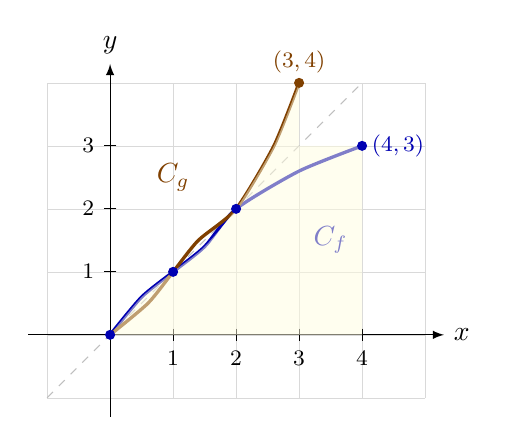
\begin{tikzpicture}[scale=0.8]
  \draw[help lines, gray!30] (-1,-1) grid (5,4);
  \draw[-latex] (-1.3,0) -- (5.3,0) node[right] {$x$};
  \draw[-latex] (0,-1.3) -- (0,4.3) node[above] {$y$};
  \foreach \x in {1,2,3,4}
    \draw (\x,0.1) -- (\x,-0.1) node[below,font=\footnotesize] {$\x$};
  \foreach \y in {1,2,3}
    \draw (0.1,\y) -- (-0.1,\y) node[left,font=\footnotesize] {$\y$};
  \draw[dashed, gray!50] (-1,-1) -- (4,4);
  % f: concave, below diagonal
  \draw[very thick, blue!70!black, smooth, tension=0.4]
    plot coordinates {(0,0) (0.5,0.6) (1,1) (1.5,1.4) (2,2) (3,2.6) (4,3)};
  \node[blue!70!black] at (3.5,1.5) {$C_f$};
  % g = f^{-1}: convex, above diagonal
  \draw[very thick, orange!50!black, smooth, tension=0.4]
    plot coordinates {(0,0) (0.6,0.5) (1,1) (1.4,1.5) (2,2) (2.6,3) (3,4)};
  \node[orange!50!black] at (1,2.5) {$C_g$};
  % shaded between
  \fill[yellow!12, opacity=0.5, smooth, tension=0.4]
    plot coordinates {(0,0) (0.5,0.6) (1,1) (1.5,1.4) (2,2) (2.6,3) (3,4)}
    -- (3,3) -- plot[smooth, tension=0.4] coordinates {(3,3) (4,3)} -- (4,3)
    -- (4,0) -- cycle;
  \filldraw[blue!70!black] (0,0) circle (2pt);
  \filldraw[blue!70!black] (1,1) circle (2pt);
  \filldraw[blue!70!black] (2,2) circle (2pt);
  \filldraw[blue!70!black] (4,3) circle (2pt) node[right,font=\footnotesize] {$(4,3)$};
  \filldraw[orange!50!black] (3,4) circle (2pt) node[above,font=\footnotesize] {$(3,4)$};
\end{tikzpicture}
\end{center}

\begin{erwthma}
  \item Εφαρμόστε Θ.Μ.Τ. στη $f$ στο $[0, 4]$ και στη $g$ στο $[0, 3]$. Υπάρχουν $\xi_f, \xi_g$ ώστε $f'(\xi_f) = \frac{3}{4}$ και $g'(\xi_g) = \frac{4}{3}$. Δείξτε ότι $f'(\xi_f) \cdot g'(\xi_g) = 1$.
  \item Υπολογίστε $\dint_0^4 f(x)\,dx + \dint_0^3 g(y)\,dy$. Τι ισούται; 
  \item Θεωρήστε $h(x) = f(x) + g(x) - 2x$ στο $[0, 3]$. Δείξτε ότι $h(0)=h(1)=h(2)=0$ και εφαρμόστε επαναληπτικά Rolle για να δείξετε ότι η $h''$ μηδενίζεται σε κάποιο $\xi \in (0, 2)$. 
  \item Αν η $f$ είναι κοίλη (κυρτή άνω) στο $[0, 4]$, δείξτε ότι $\dint_0^4 f(x)\,dx \leq \frac{f(0)+f(4)}{2} \cdot 4 = 6$ και χρησιμοποιήστε τη σχέση ολοκληρωμάτων για να δείξετε ότι $\dint_0^3 g(y)\,dy \geq 6$.
\end{erwthma}
\end{thema}
